% Metódy inžinierskej práce

\documentclass[10pt,twoside,slovak,a4paper]{article}

\usepackage[slovak]{babel}
\usepackage {float}
%\usepackage[T1]{fontenc}
\usepackage[IL2]{fontenc} 
\usepackage[utf8]{inputenc}
\usepackage{graphicx}
\usepackage{url} % príkaz \url na formátovanie URL
\usepackage{hyperref} % odkazy v texte budú aktívne (pri niektorých triedach dokumentov spôsobuje posun textu)

\usepackage{cite}
%\usepackage{times}

\pagestyle{headings}

\title{Vývin inovatívnej platformy e-learningu pre nepočujúcich\thanks{Semestrálny projekt v predmete Metódy inžinierskej práce, ak. rok 2020/21, vedenie: Ing. Ján Lang, PhD.}} % meno a priezvisko vyučujúceho na cvičeniach

\author{Petra Hlavinová\\[2pt]
	{\small Slovenská technická univerzita v Bratislave}\\
	{\small Fakulta informatiky a informačných technológií}\\
	{\small \texttt{xhlavinova@stuba.sk}}
	}

\date{\small 15. október 2020} % upravte



\begin{document}

\maketitle

\begin{abstract}
E-learning je čoraz viac atraktívnejším nástrojom pre študentov. Vďaka neustálemu rozširovaniu inteligentných zariadení a modernej technológie sa stáva učenie a získavanie informácií stále jednoduchšie a rýchlejšie. Práve pre nepočujúcich študentov môže mať e-learning množstvo výhod, no napriek tomu čelí táto skupina so špecifickými vzdelávacími potrebami v dnešnej dobe mnohým prekážkam v prístupe ku vzdelávaniu. V tejto štúdii sme sa zamerali na skúmanie týchto prekážok, spôsobu, akým sa nepočujúci učia, ako aj na to, ako by im mali byť prezentované informácie a najmä vzdelávací obsah. Naším cieľom bolo analyzovať kognitívne vlastnosti nepočujúcich a hlavne nájsť a vyvinúť inovatívnu a užívateľský prívetivú platformu e-learningu vhodnú pre potreby nepočujúcich študentov. 
\end{abstract}



\section{Úvod}
\centering
Zdá sa, že nepočujúci ľudia sú v dnešnej dobe stále do veľkej miery sociálne vylúčení. Sociálne vylúčenie nepočujúcich je podmienené viacerými faktormi, či už vzdelávacím systémom, hospodárskou politikou, právnymi predpismi v sociálnej oblasti a postojmi ľudí v spoločnosti. Paradoxne však práve celoživotné vzdelávanie predstavuje rozhodujúci parameter proti sociálnemu vylúčeniu nepočujúcich ľudí. Vznik e-learningu uľahčil vzdelávanie pre ľudí na celom svete. Sila internetu, a teda aj e-learning, spočíva v jeho univerzálnosti. Z toho vyplýva, že musí byť prístupný ľuďom s rôznym rozsahom sluchu, zraku, pohybu a kognitívnych schopností.  V minulosti sa však zvyklo myslieť, že nepočujúcim stačí na uchopenie informácií písomný prepis zvukového obsahu. Práve toto predstavuje hlavný problém pri vzdelávaní tejto cieľovej skupiny, ktorému sa budeme potrebnejšie venovať v kapitole číslo ~\ref{rozdiely} .Práve preto, aby e-vzdelávanie pokrylo túto medzeru v gramotnosti, sú potrebné kreatívne spôsoby prezentácie a koordinácie interaktívnych vizuálnych materiálov.
Dôležité súvislosti sú uvedené v častiach~\ref{dolezita} a~\ref{dolezitejsia}.
Záverečné poznámky prináša časť~\ref{zaver}.



\section{Vplyv internetu na skupinu sluchovo postihnutých} \label{vplyvinternetu}

\begin{flushleft}
	Podľa World Wide Web Consortium bol internet navrhnutý tak, aby fungoval pre všetkých jednotlivcov bez ohľadu na ich schopnosti. Vplyv internetu zásadne mení prístup k vzdelávaniu pre nepočujúcich, pretože jeho použitie \emph{odstraňuje komunikačné a interakčné bariéry}, ktorým môžu jednotlivci vo fyzickom svete čeliť. To zdôrazňuje potrebu poskytnúť ľuďom so zdravotným postihnutím príležitosti bez ohľadu na ich zdravotné postihnutie sprístupnením online služieb, najmä e-learningu, spôsobom, ktorý rešpektuje a zohľadňuje ich potreby. Nejde len o rovnaké ľudské práva, ale aj o to, aby táto technológia a jej výhody mali mať úžitok aj pre nepočujúcich a sluchovo postihnutých ľudí. Inak provokuje fenomén „digitálnej priepasti“.Citované z \cite{pappas2018learning}
	\end{flushleft}
	\footnote{World Wide Web Consortium (W3C) je medzinárodné konzorcium, ktorého členovia spoločne s verejnosťou vyvíjajú webové štandardy pre World Wide Web.\cite{WWWC}}
	\clearpage

\section{Rozdiely v kognitívnych funkciách medzi nepočujúcimi a počujúcimi jedincami} \label{rozdiely}
Vývin vhodnej e-learningovej platformy pre nepočujúcich by sa mal realizovať v súlade s učebným profilom, ako aj so špecifickými vzdelávacími potrebami  tejto cieľovej skupiny. Z tohto dôvodu je potrebné v prvom rade preskúmať hlavné rozdiely v kognitívnych schopnostiach medzi nepočujúcimi a počujúcimi jedincami.\linebreak
Tieto rozdiely môžeme rozdeliť do následovných sfér:
\begin{itemize}
\item ~\ref{rozdiely:vseob} Všeobecný kognitívny profil
\item ~\ref{rozdiely:pozornost} Pozornosť
\item ~\ref{rozdiely:pamat} Práca s pamäťou
\item ~\ref{rozdiely:citanie} Čítanie s porozumením
\end{itemize}
Základným problémom je teda\ldots{} Najprv sa pozrieme na nejaké vysvetlenie (časť~\ref{ina:nejake}), a potom na ešte nejaké (časť~\ref{ina:nejake}).\footnote{Niekedy môžete potrebovať aj poznámku pod čiarou.}
Dôležité veci možno \emph{zdôrazniť kurzívou}.


\subsection{Všeobecný kognitívny profil} \label{rozdiely:vseob}
Priemerné skóre IQ nepočujúcich je porovnateľné s počujúcimi jednotlivcami a má tendenciu sa časom zvyšovať. Nepočujúci jedinci však vykazujú rozdiely v porovnaní s počujúcimi rovesníkmi, pokiaľ ide o ich pamäť, zručnosti pri riešení problémov a akademické výsledky. Vizuálne komunikačné schopnosti nepočujúcich, ako napríklad spracovanie vizuálneho jazyka, predstavujú individuálne kognitívne rozdiely. Uvádza sa, že nepočujúci a sluchovo postihnutí jedinci majú rovnakú úroveň citlivosti na vizuálny kontrast. Okrem toho sa zdá, že nepočujúce deti majú poruchy jemného motorického sekvenovania, a to napriek skutočnosti, že ich vizuopriestorové kognitívne schopnosti sa výrazne nelíšia od ich sluchových vrstovníkov.
Citované z \cite{pappas2018learning}


\subsection{Pozornosť} \label{rozdiely:pozornost}
Pozornosť je rozhodujúca pre každodenné činnosti nepočujúcich jedincov, pretože identifikácia periférnych vizuálnych znakov je pre nich dôležitejšia z dôvodu straty sluchu. Strata sluchu sa nepovažuje za prediktívny faktor deficitov pozornosti, pretože nepočujúci jedinci majú v porovnaní so svojimi počujucími rovesníkmi rovnaké a niekedy dokonca aj lepšie výsledky pri riešení úloh vyžadujúcich pozornosť. Avšak existujú aj dôkazy o významných rozdieloch vo vizuálnej pozornosti, najmä v periférnej pozornosti. Štúdia Baveliera, Dyeho a Hausera (2006) odhalila, že nepočujúci jedinci sú viac rozptýlení periférnymi rušičmi a menej centrálnymi rušičmi.
Citované z \cite{bavelier2006deaf} a \cite{pappas2018learning}.

\subsection{Práca s pamäťou} \label{rozdiely:pamat}
Zdá sa, že včasné vystavenie posunkovej reči má pozitívny vplyv na kognitívny vývoj nepočujúcich detí, ako aj na zvládnutie vizuálnych perspektív. Napriek tomu však existujú dôkazy, že medzi nepočujúcimi a počujúcimi jedincami sú rozpoznateľné rozdiely pri práci s pamäťou. Tieto rozdiely vyplývajú zo skutočnosti, že zapamätávanie pomocou posunkového jazyka vyžaduje viac miesta v pamäti ako prostredníctvom hovoreného jazyka. Posunkové jazyky môžu mať negatívny vplyv na krátkodobú pamäť kvôli ich vizuopriestorovej povahe. 
Citované z \cite{pappas2018learning}.
\begin{figure}[H]
	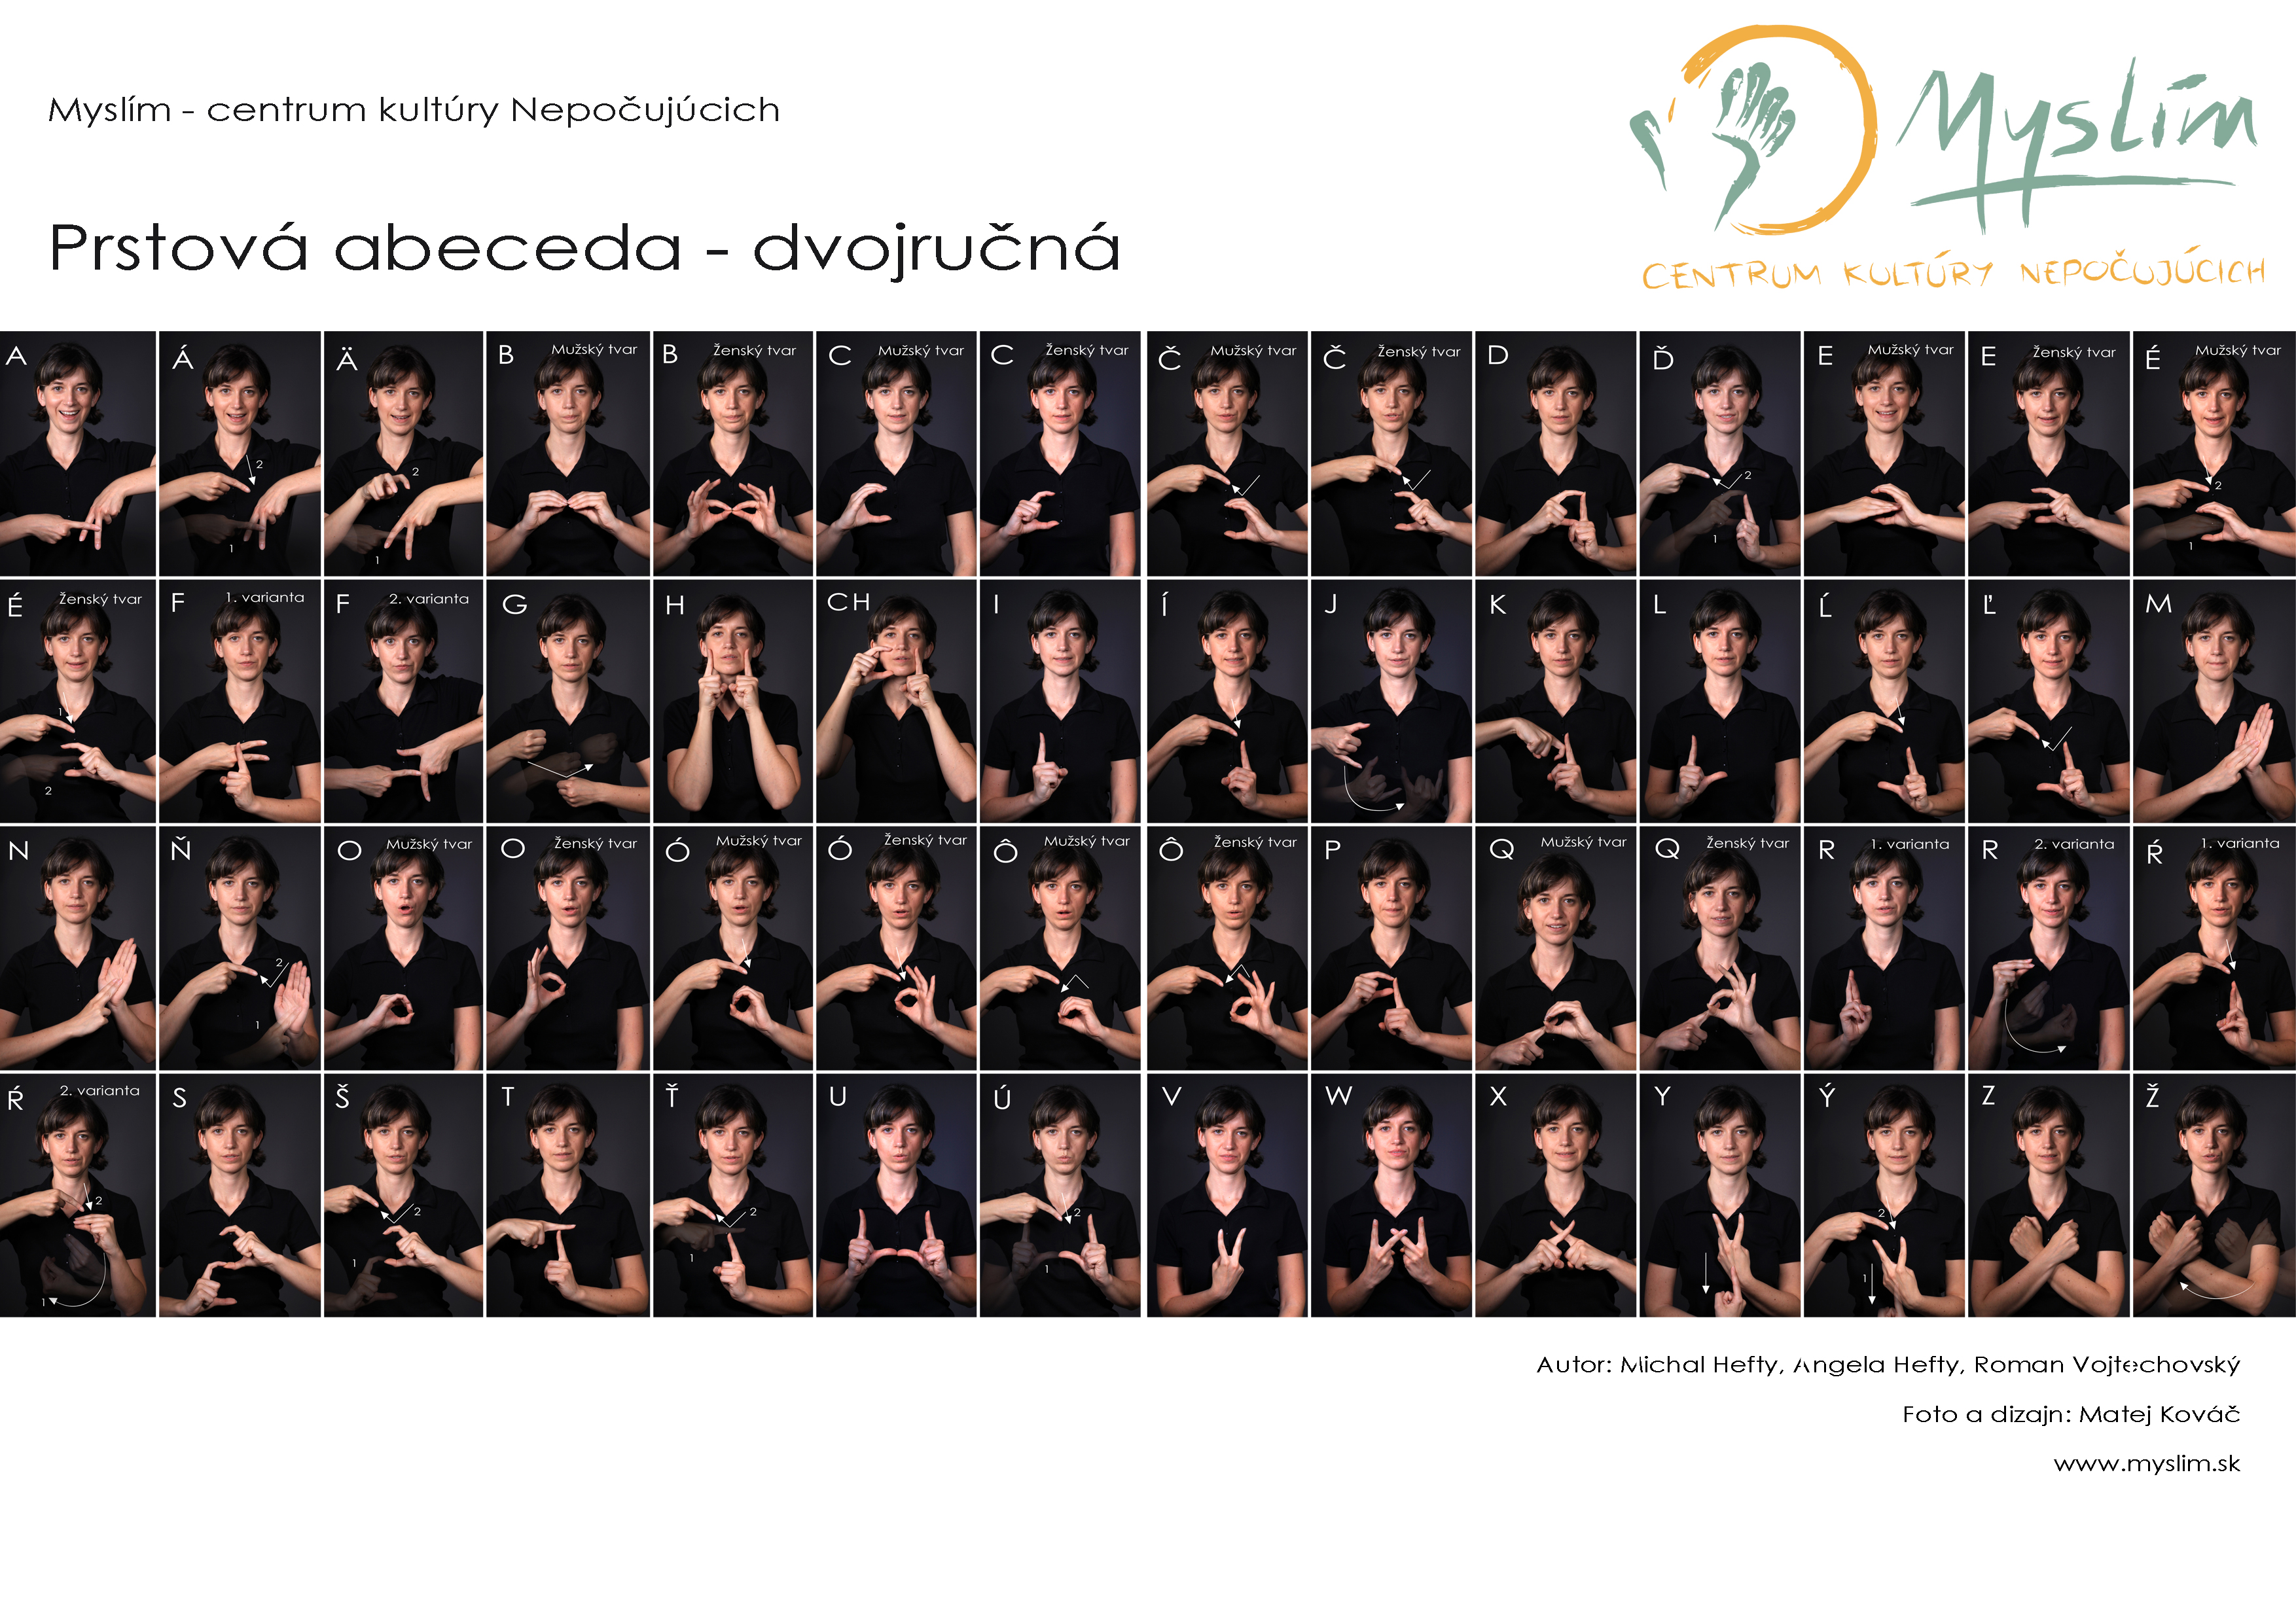
\includegraphics[scale=0.1]{dvojrucna-tlac.jpg}
 \centering
 \caption{Slovenská prstová abeceda - dvojručná.}
 \cite{mytyafakty}
 \label{slovenskaposunkovarec}
 \end{figure}
 

\subsection{Čítanie s porozumením} \label{rozdiely:citanie}
Nepočujúci majú nízku úroveň čitateľských schopností, pretože majú odlišný spôsob rozpoznávania slov v porovnaní s počujúcimi čitateľmi. Porozumenie textu nepočujúcich dospelých súvisí s ich čitateľskou motiváciou, a tak by práve náročné materiály na čítanie mohli postupne zlepšovať ich čitateľské schopnosti. Domínguez a Alegria (2009) skúmali mechanizmy čítania, ktoré používajú nepočujúci dospelí. Výsledky ukázali, že väčšina účastníkov používa na pochopenie textu stratégiu kľúčových slov. 
 Citované z \cite{pappas2018learning} a \cite{dominguez2010reading}

 \section{Navrhovanie e-learningových systémov} \label{dolezita}
 Špeciálne vzdelávacie potreby osôb so zdravotným postihnutím, ako je hluchota a čiastočná strata sluchu, sa žiaľ dodnes pri vývoji systémov elektronického vzdelávania zohľadňujú zriedka. Je pravda, že návrh rozhraní, ktoré sú pre nich vhodné a užívateľsky prívetivé, nie je vždy ľahký proces. Jazykové a gramotné schopnosti sa môžu líšiť v závislosti od typu a úrovne hluchoty a veku človeka, ktorý stratil sluch, a môžu byť ovplyvnené zároveň aj ich schopnosti čítania a písania. To vyvoláva problémy pri vytváraní e-learningových rozhraní. Projektanti takýchto systémov musia zohľadňovať špeciálne potreby cielovej skupiny, ktoré sa vyskytujú na komunikačnej aj kognitívnej úrovni.
 Citované z \cite{pappas2018learning}




\section{Ešte dôležitejšia časť} \label{dolezitejsia}




\section{Záver} \label{zaver} % prípadne iný variant názvu



%\acknowledgement{Ak niekomu chcete poďakovať\ldots}


% týmto sa generuje zoznam literatúry z obsahu súboru literatura.bib podľa toho, na čo sa v článku odkazujete
\bibliography{literatura}
\bibliographystyle{plain} % prípadne alpha, abbrv alebo hociktorý iný
\end{document}
